%%
%% Приложение 3. Печатная плата управляющего устройства.
%% Copyright (C) 2011 Alex Anisimov, <zolkko@gmail.com>
%%

\documentclass[russian,utf8,a1paper,landscape]{eskdgraph}
\usepackage{mathtext}
\usepackage[T2A]{fontenc}
\usepackage[russian]{babel}
\usepackage{mathptmx}
\usepackage{amstext}
\usepackage{amsmath}
\usepackage{amssymb}
\usepackage{ltxtable}
\usepackage{multirow}
\usepackage{tabularx}
\usepackage{array}
\usepackage{textcomp}
\usepackage{lscape}
\usepackage{rotating}
\usepackage{geometry}
\graphicspath{{/Users/zolkko/Projects/zolkko-alarm/doc/imgs/}}
\usepackage{listings}
\usepackage{float}
\usepackage{pscyr}

\renewcommand{\ESKDfontVsize}{\fontsize{13pt}{14pt}}

\ESKDcolumnI{Печатная плата управляющего устройства универсальной системы терморегулирования}
\ESKDcolumnII{ДП 508441 02}
\ESKDcolumnVI{1:2.4}
\ESKDcolumnIX{ВГТУ}
\ESKDcolumnXIfI{\small{Анисимов А. Н.}}
\ESKDcolumnXIfII{\small{Барабанов В.Ф.}}

\begin{document}
	\begin{ESKDdrawing}
		\center{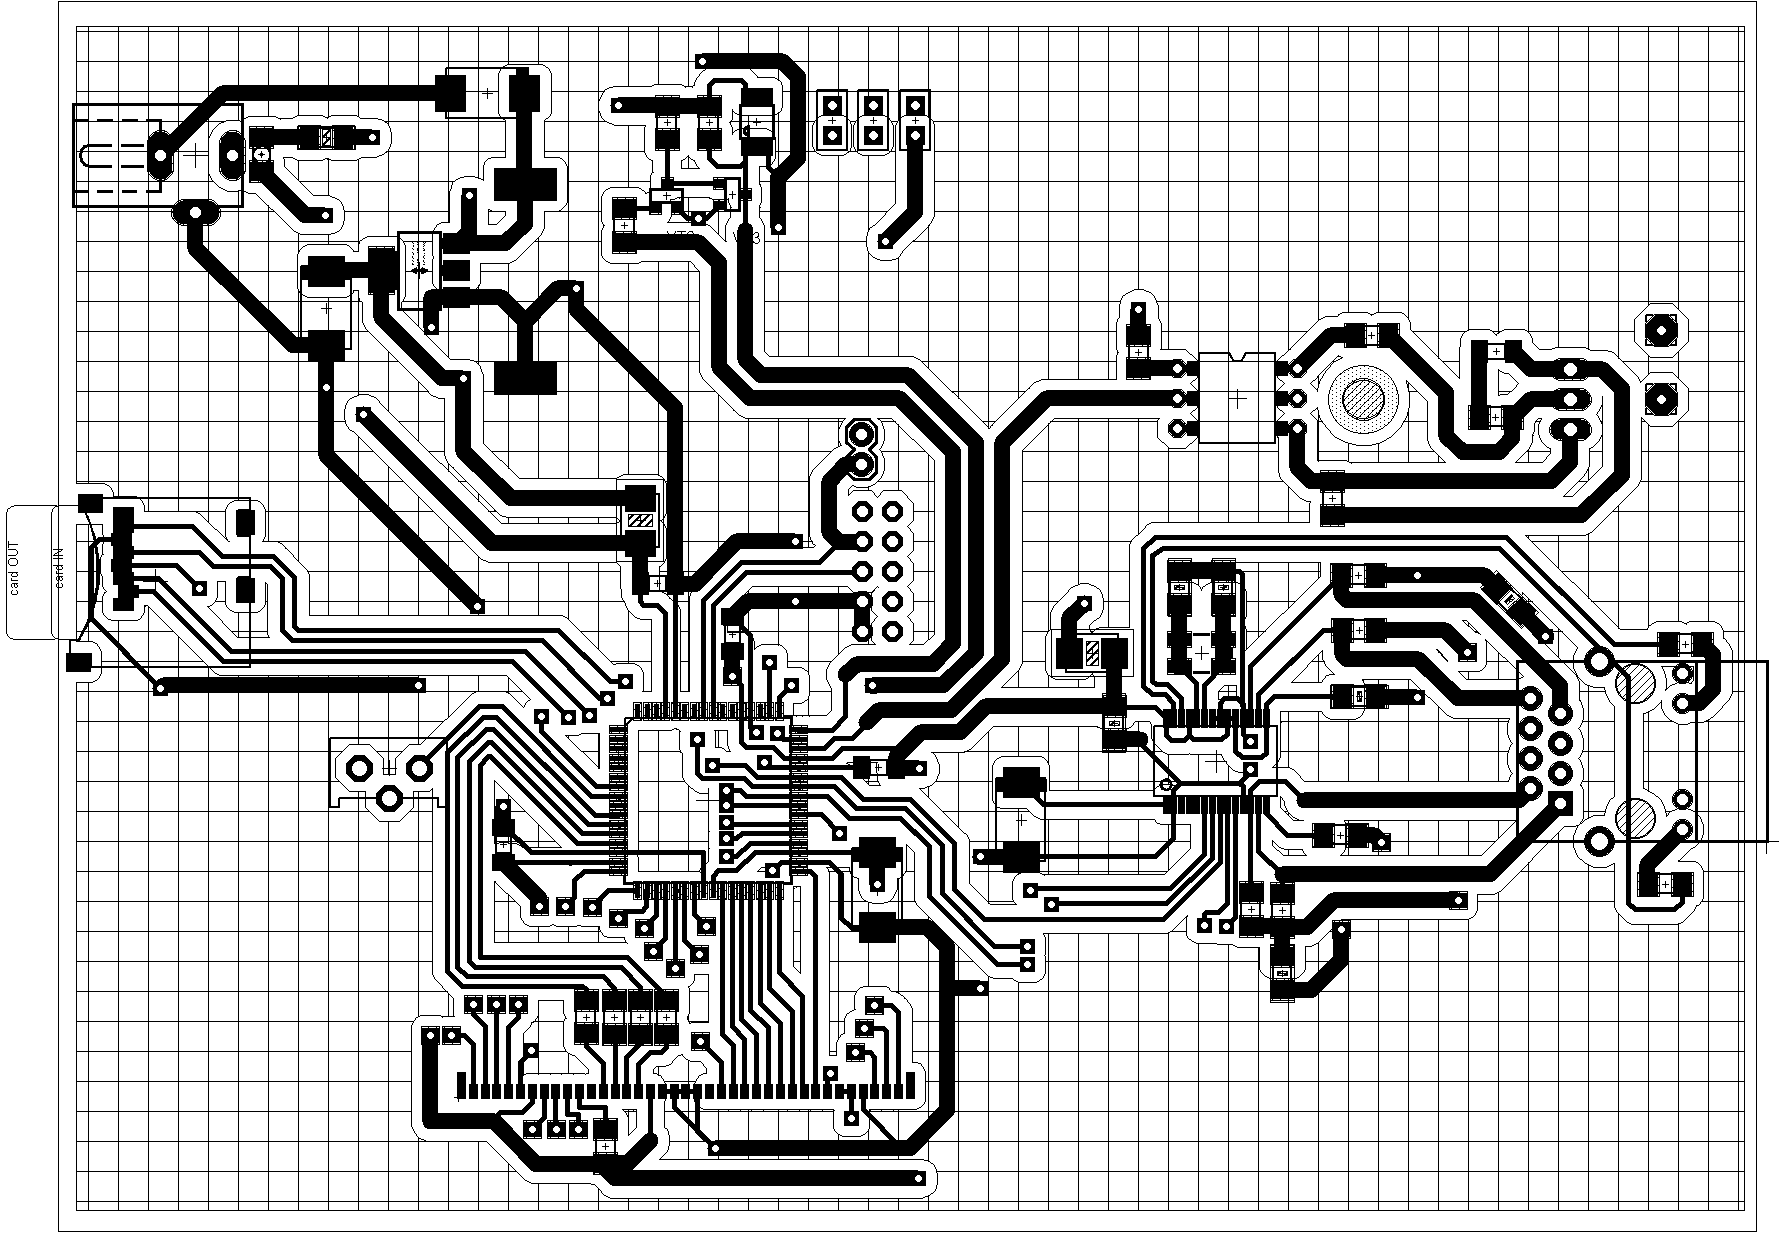
\includegraphics[bb=0 0 430 320, clip, scale=2.4]{pcb_top_mono.png}}
		\center{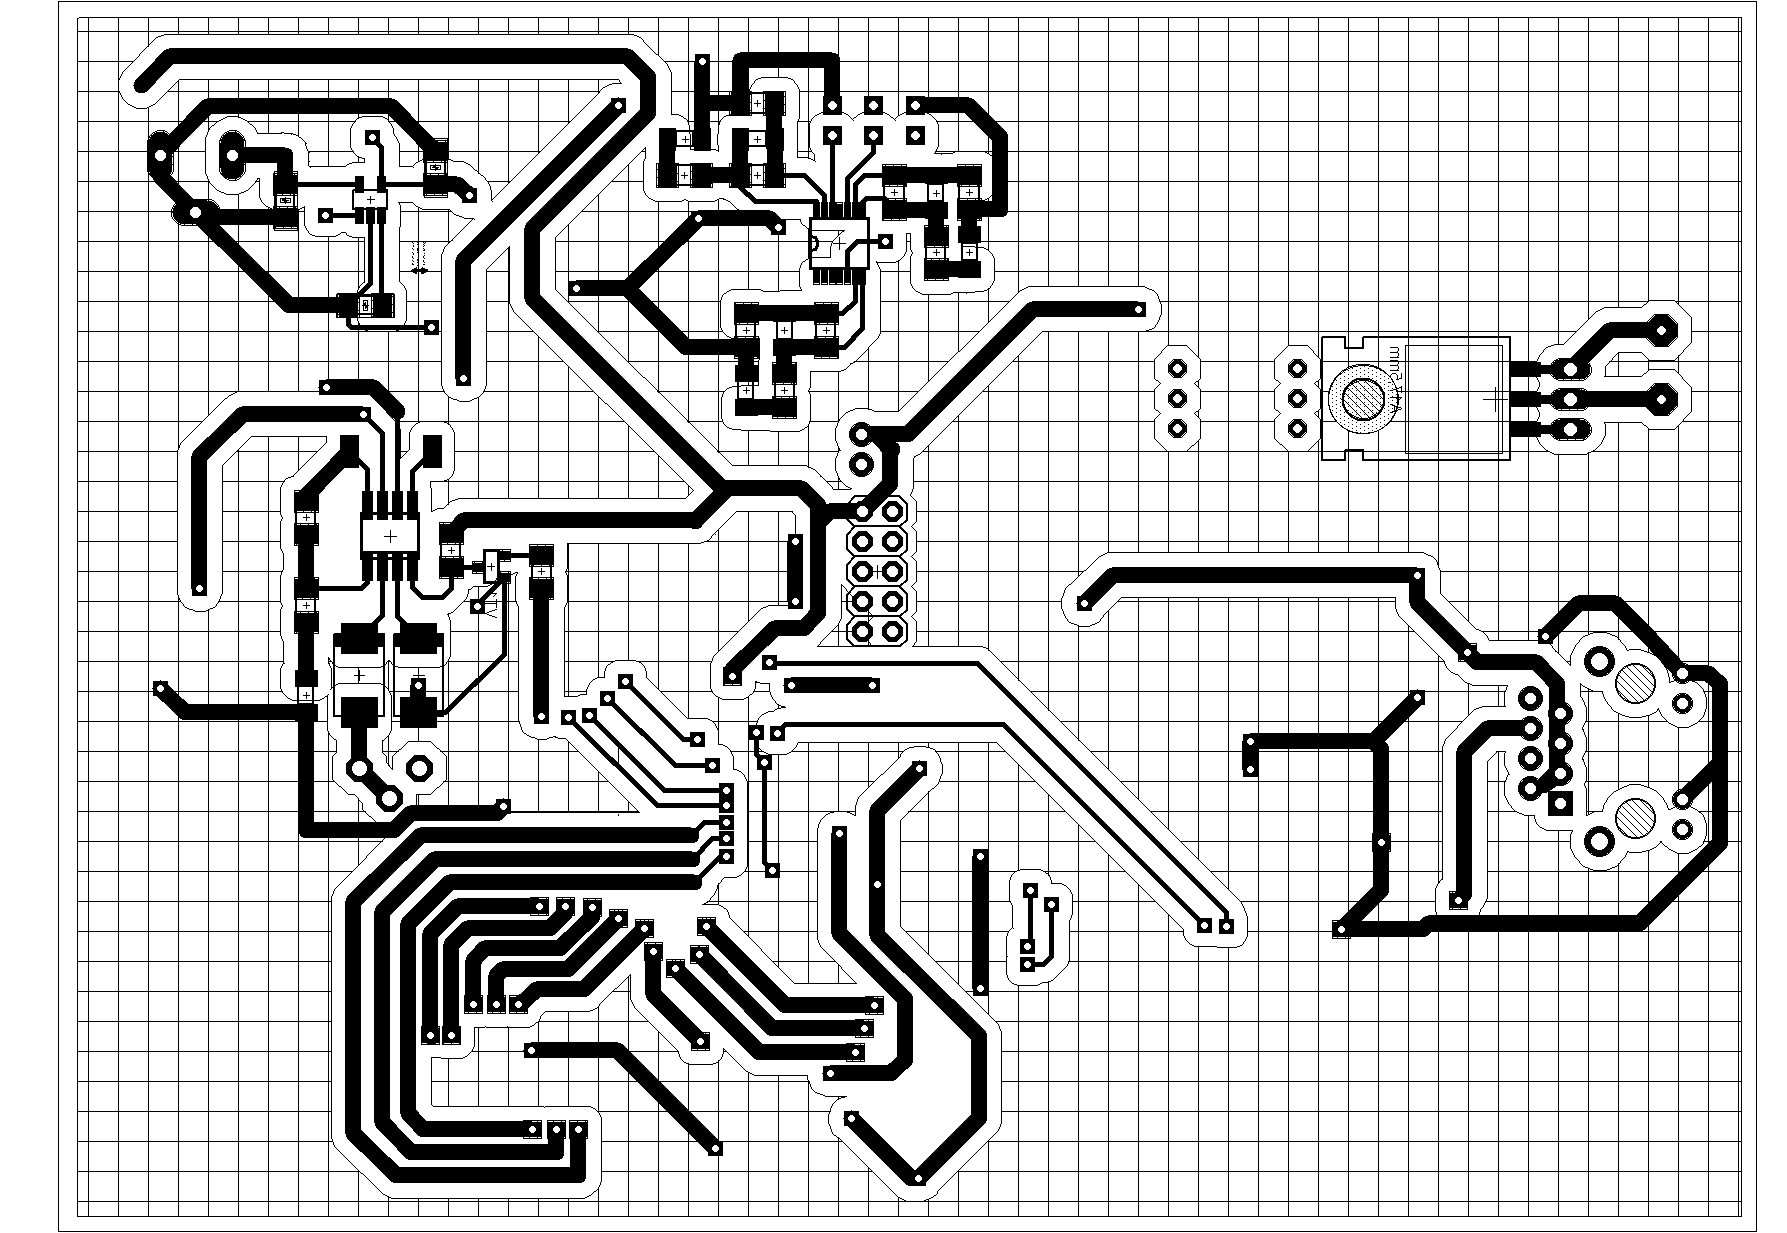
\includegraphics[bb=0 0 430 320, clip, scale=2.4]{pcb_bottom_mono.png}}
	\end{ESKDdrawing}
\end{document}
